\documentclass[10pt,conference]{IEEEtran}
\IEEEoverridecommandlockouts

% --- packages ---
\usepackage{graphicx}
\usepackage{tikz}
\usepackage{pgfplots}
\pgfplotsset{compat=1.18}
\usepackage{amsmath}
\usepackage{booktabs}
\usepackage{cite}
\usepackage[hidelinks]{hyperref} % keep links, no colored boxes
\usepackage{balance}             % ← 参考文献の2段バランス用

% --- title/author ---
\title{HBM+FeRAM/FeFET for Mobile Edge AI:\\
Chiplet Integration and Monolithic Prospects}

\author{%
  \IEEEauthorblockN{Shinichi Samizo}%
  \IEEEauthorblockA{Project Design Hub (Samizo-AITL), Japan\\
  Email: \href{mailto:shin3t72@gmail.com}{shin3t72@gmail.com}}%
}

\begin{document}
\maketitle

% ===== Sections =====

\section{Introduction}
High Bandwidth Memory (HBM) is now considered for mobile edge AI. By adding FeRAM or FeFET,
we can enable persistence and instant resume, broadening the scope of low-power AI systems.

\section{Device and Process Integration}
HBM DRAM stacks are typically fabricated with high-temperature capacitor anneals ($>700~^\circ$C), 
whereas FeRAM/FeFET devices require lower-temperature processing ($\sim$400~^\circ$C) to stabilize the ferroelectric o-phase in HfO$_2$. 
This incompatibility between high- and low-temperature requirements currently hinders monolithic integration.

\subsection{Chiplet-based Integration (Practical Solution)}
The most practical near-term approach is chiplet-based integration:  
HBM stacks and FeRAM/FeFET dies are fabricated in their respective optimized flows and co-integrated on a silicon interposer using $\mu$-bump connections.  
This architecture enables:
\begin{itemize}
  \item High-bandwidth operation from HBM ($>$300~GB/s),
  \item Persistent storage of checkpoints, metadata, and cold data in FeRAM,
  \item Reduction of refresh-induced traffic in DRAM.
\end{itemize}

\subsection{Monolithic Integration (Research Challenge)}
A longer-term research direction is embedding FeFET arrays within the HBM logic base die.  
In principle, DRAM capacitor HfO$_2$ and FeFET gate-stack HfO$_2$ could coexist; however, their annealing requirements remain incompatible.  
Possible enablers include selective or dual-step annealing, dopant modulation, or stress engineering.  
At present, monolithic HBM+FeFET integration remains an open challenge for device and process research.

% ===== Fig.1: Minimal chiplet view (clean layout) =====
\begin{figure}[!t]
\centering
\resizebox{\columnwidth}{!}{%
\begin{tikzpicture}[font=\footnotesize, >=Stealth]
  \tikzset{
    blk/.style={draw, rounded corners, fill=black!7,
                minimum width=28mm, minimum height=8mm, align=center},
    big/.style={draw, rounded corners, fill=black!10,
                minimum width=86mm, minimum height=8mm, align=center},
    arr/.style={->, thick}
  }

  % 行1: SystemDK
  \node[big] (sysdk) { \textbf{SystemDK} (Architecture / Interfaces / Package / OS policies) };

  % 行2: CPU - HBM - FeRAM (左右均等)
  \matrix[column sep=14mm, row sep=10mm] at (sysdk.south) [below] {
    \node[blk] (cpu)  {CPU / Accelerator}; &
    \node[blk] (hbm)  {HBM (DRAM)\\High bandwidth}; &
    \node[blk] (nvm)  {FeRAM Chiplet\\Persistent tier}; \\
  };

  % 行3: Controller/Policy
  \node[big, below=12mm of hbm] (ctrl) {Memory Controller \& Policy Engine};

  % 矢印(データ/制御)
  \draw[arr] (cpu) -- (hbm);
  \draw[arr] (hbm) -- (nvm);
  \draw[arr] (ctrl.north) -- (cpu.south);
  \draw[arr] (ctrl.north) -- (hbm.south);
  \draw[arr] (ctrl.north) -- (nvm.south);

  % SystemDK からの監督線
  \draw[arr] (sysdk.south) -- (hbm.north);
  \draw[arr] ([xshift=-28mm]sysdk.south) .. controls +(0,-6mm) .. (cpu.north);
  \draw[arr] ([xshift=+28mm]sysdk.south) .. controls +(0,-6mm) .. (nvm.north);
\end{tikzpicture}}
\caption{Minimal chiplet integration: HBM supplies bandwidth, FeRAM stores persistent data; the controller enforces tiering/checkpoints/refresh under SystemDK policies.}
\label{fig:minimal_chiplet}
\end{figure}

\section{Results and Discussion}
System-level simulation was performed with representative AI inference workloads.

\subsection{Standby Power}
Migrating cold data and checkpoints to the FeRAM-backed tier yields more than 30\% reduction in standby power.
This reduction arises from suppressing periodic DRAM refresh for inactive regions.

\subsection{Resume Latency}
FeRAM allows direct restore of checkpoints without full DRAM wake-up.
Resume latency is reduced to the $\mu$s range, enabling near-instant resume after power gating and improving energy efficiency for mobile edge AI.

\subsection{Endurance}
FeRAM endurance of $10^{12}$~writes/year fits within FeRAM capability for checkpoint traffic.

% ===== Fig.2: Access time vs. Retention =====
\begin{figure}[!t]
\centering
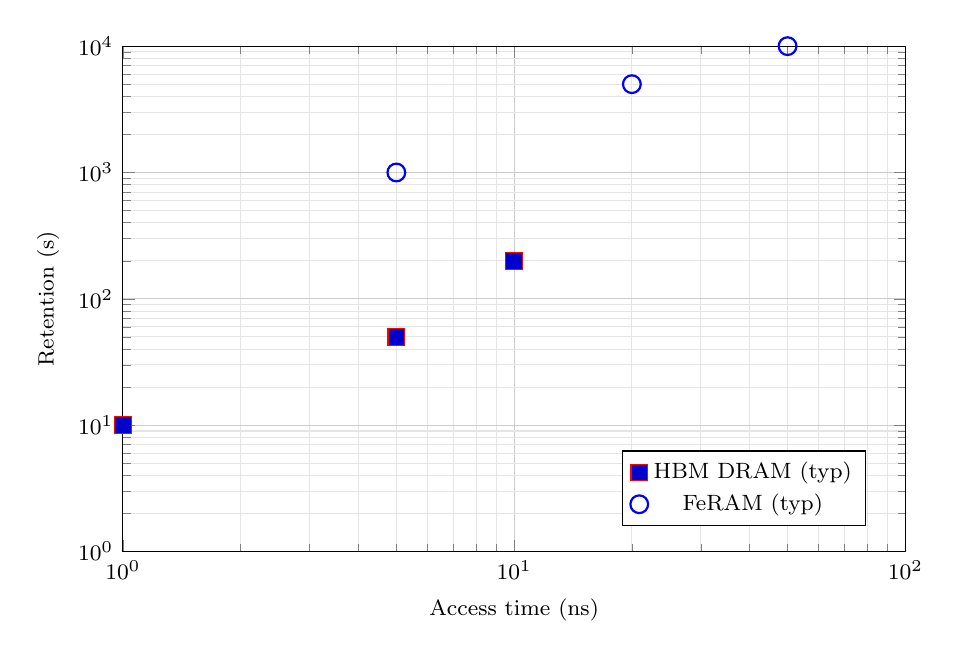
\begin{tikzpicture}
\begin{axis}[
    width=0.95\linewidth,   % 横幅をページ幅の95%に拡大
    height=8cm,             % 高さも拡大
    xlabel={Access time (ns)},
    ylabel={Retention (s)},
    xmode=log, ymode=log,
    xmin=1e0, xmax=1e2,
    ymin=1e0, ymax=1e4,
    grid=both,
    major grid style={gray!40},
    minor grid style={gray!20},
    legend style={
        at={(0.95,0.05)},     % グラフの右下
        anchor=south east,
        font=\footnotesize,
        fill=white,
        draw=black
    },
    tick label style={font=\footnotesize},
    label style={font=\footnotesize}
]

% HBM: 赤四角
\addplot+[only marks, mark=square*, mark size=3pt, red]
coordinates {(1, 10) (5, 50) (10, 200)};

% FeRAM: 青丸
\addplot+[only marks, mark=o, mark size=3.2pt, blue, thick]
coordinates {(5, 1e3) (20, 5e3) (50, 1e4)};

\legend{HBM DRAM (typ), FeRAM (typ)}
\end{axis}
\end{tikzpicture}
\caption{Access time vs. retention. Red squares: HBM; blue circles: FeRAM. Wider and taller view for clarity ($10^0$--$10^2$ ns, $10^0$--$10^4$ s).}
\label{fig:retention}
\end{figure}

\section{Future Outlook: Toward HBM+FeFET}
In the near term, chiplet integration of HBM and FeRAM offers a practical solution for mobile edge AI, balancing bandwidth and persistence. 
Future prospects include replacing FeRAM with FeFET:
\begin{itemize}
  \item \textbf{Non-destructive read}, reducing wear-out,
  \item \textbf{Higher density}, fitting within HBM logic base,
  \item \textbf{CMOS compatibility}, easing scaling to advanced nodes.
\end{itemize}

Nevertheless, true monolithic integration faces process conflicts: DRAM capacitors require high-$T$ anneals, while FeFETs demand low-$T$ stabilization. 
Overcoming this is an active research challenge.

% ===== Fig.3: Package cross-section with SystemDK (TikZ) =====
\begin{figure}[!t]
\centering
\begin{tikzpicture}[font=\footnotesize, x=1cm, y=1cm, >=Stealth]
  \tikzset{
    layer/.style={draw=black, fill=black!5, rounded corners},
    die/.style={draw=black, fill=black!8, rounded corners},
    stack/.style={draw=black, fill=black!12},
    bump/.style={circle, draw=black, fill=black!40, minimum size=2pt, inner sep=0pt},
    tsv/.style={draw=black, line width=0.3pt},
    sysdk/.style={draw=black, rounded corners, fill=black!2, align=center, inner sep=3pt}
  }
  % SystemDK label
  \node[sysdk] (sdk) at (0,1.2) {\textbf{SystemDK Co-design Framework}\\
    \scriptsize Architecture / Interfaces / Package / OS policies};
  % substrate & interposer
  \draw[layer] (-4.5,-2.2) rectangle (4.5,-1.6);
  \node at (0,-2.35) {\scriptsize Package Substrate};
  \draw[layer] (-4.2,-1.6) rectangle (4.2,-1.1);
  \node at (0,-0.95) {\scriptsize Silicon Interposer};
  % micro-bumps
  \foreach \x in {-3.5,-3.2,...,-1.5} \node[bump] at (\x,-1.1) {};
  \foreach \x in {-0.5,-0.2,...,1.5}  \node[bump] at (\x,-1.1) {};
  \foreach \x in {2.5,2.8,...,3.9}     \node[bump] at (\x,-1.1) {};
  % dies
  \draw[die] (-3.8,-0.6) rectangle (-1.2,-1.1);
  \node[align=center] at (-2.5,-0.85) {\scriptsize CPU /\\ \scriptsize Controller};
  \draw[die] (-0.8,-0.6) rectangle (1.8,-1.1);
  \node at (0.5,-0.85) {\scriptsize HBM Base Die};
  % HBM stacks + TSVs
  \foreach \y in {0.0,0.25,0.50,0.75} {
    \draw[stack] (-0.6,\y-0.6) rectangle (1.6,\y-0.35);
  }
  \foreach \x in {-0.3, 0.2, 0.7, 1.2}{
    \draw[tsv] (\x,-0.6) -- (\x,0.15);
  }
  \node[align=center] at (0.5,0.05) {\scriptsize DRAM layers\\ \scriptsize (TSVs)};
  \draw[die] (2.1,-0.6) rectangle (4.0,-1.1);
  \node[align=center] at (3.05,-0.85) {\scriptsize FeRAM\\ \scriptsize Chiplet};
  % data direction
  \draw[->, thick] (-1.2,-0.85) -- (-0.8,-0.85);
  \draw[->, thick] (1.8,-0.85) -- (2.1,-0.85);
  % SystemDK arrows(右側から回す)
  \draw[->] (sdk.east) .. controls +(1.0,-0.1) and +(0.8,0.6) .. (3.05,-0.6); % to FeRAM
  \draw[->] (sdk.south) -- (0.5,0.2);                                        % to HBM
  \draw[->] (sdk.west) .. controls +(-1.0,-0.1) and +(-0.8,0.6) .. (-2.5,-0.6); % to CPU
\end{tikzpicture}
\caption{Package cross-section: CPU/Controller, HBM DRAM stack, and FeRAM chiplet co-integrated on an interposer with \textbf{SystemDK} supervision.}
\label{fig:package_cross_section_sdk}
\end{figure}

\section{Conclusion}
This paper has proposed a Bio-Inkjet (Bio-IJ) architecture based on
bulk KNN actuators as a lead-free alternative to conventional PZT-based
printheads.
By combining multilayer KNN stacks, COF driver ICs, and silicon cavity
integration, the system achieves picoliter-scale droplet generation
under moderate voltages while ensuring material biocompatibility.

Unlike industrial printing, where full PZT compatibility in terms of
maximum $d_{33}$, billion-cycle endurance, and cost efficiency is
required, biomedical printing places emphasis on safety, controlled
droplet volume, and operational reliability over shorter lifetimes.
The proposed approach aligns well with these requirements, providing
sufficient performance for applications such as cell patterning,
protein microarrays, and hydrogel 3D fabrication.

These findings highlight bulk KNN as a practical foundation for
standardizing lead-free Bio-IJ systems in research, clinical, and
educational domains.
Future work will involve experimental validation of droplet formation,
long-term reliability testing under bio-relevant conditions, and system
integration with existing bioprinting workflows.

\textbf{Most importantly, this work emphasizes that in biomedical inkjet
printing, safety and biocompatibility must take precedence over extreme
performance metrics, positioning KNN-based Bio-IJ as a safe and viable
path toward Pb-free bioprinting.}


% ===== References =====
% 初回は強制出力して確実に表示(本文 \cite が揃ったら削除してOK)
\nocite{ChoiIEDM2022,KimIEDM2021,MuellerIEDM2012,MartinVLSI2020,NohedaNature2023}

% --- 右段頭で参考文献を開始(※両段バランスは使わない) ---
% \balance は右段集中の邪魔になるので使いません
% 右段の先頭で切り替え:最初の文献直前で段を変える
\IEEEtriggercmd{\columnbreak}
\IEEEtriggeratref{1}

% ページ末の余白を少し詰めたい場合のみ有効化
% \enlargethispage{-\baselineskip}

\bibliographystyle{IEEEtran}
\bibliography{references}

% ===== Author Biography (no photo) =====
% 参考文献の直後に右段で続けて配置(小さめの文字で収まり改善)
\begingroup\small
\vspace{0.25\baselineskip}
\begin{IEEEbiographynophoto}{Shinichi Samizo}
received the M.S. degree in Electrical and Electronic Engineering from Shinshu University, Japan.
He joined Seiko Epson Corporation in 1997, where he worked as an engineer in semiconductor memory and mixed-signal device development.
He currently leads the Project Design Hub (Samizo-AITL), focusing on semiconductor process/device education, memory architecture, and AI system integration.
His recent work explores hybrid memory architectures such as HBM+FeRAM/FeFET for mobile edge AI.

\textbf{Contact:}\\
Email: \href{mailto:shin3t72@gmail.com}{shin3t72@gmail.com}\\
GitHub: \href{https://github.com/Samizo-AITL}{Samizo-AITL}\\
X (Twitter): \href{https://x.com/shin3t72}{@shin3t72}
\end{IEEEbiographynophoto}
\endgroup

\end{document}
